\documentclass[frenchb, oneside, headings=normal]{scrartcl}

\usepackage[utf8x]{inputenc}
\usepackage[T1]{fontenc}
\usepackage{lmodern}

\usepackage{ifthen}
\usepackage{url}


\usepackage{multirow}

% Color
% cfr http://en.wikibooks.org/wiki/LaTeX/Colors
\usepackage{color}
\usepackage[usenames,dvipsnames,svgnames,table]{xcolor}
\definecolor{dkgreen}{rgb}{0.25,0.7,0.35}
\definecolor{dkred}{rgb}{0.7,0,0}

\newcommand{\matlab}{\textsc{Matlab}}

% Math symbols
\usepackage{amsmath}
\usepackage{amssymb}
\usepackage{amsthm}
\DeclareMathOperator*{\argmin}{arg\,min}
\DeclareMathOperator*{\argmax}{arg\,max}


% Sets
\newcommand{\Z}{\mathbb{Z}}
\newcommand{\R}{\mathbb{R}}
\newcommand{\Rn}{\R^n}
\newcommand{\Rnn}{\R^{n \times n}}
\newcommand{\C}{\mathbb{C}}
\newcommand{\K}{\mathbb{K}}
\newcommand{\Kn}{\K^n}
\newcommand{\Knn}{\K^{n \times n}}

% Unit vectors
\usepackage{esint}
\usepackage{esvect}
\newcommand{\kmath}{k}
\newcommand{\xunit}{\hat{\imath}}
\newcommand{\yunit}{\hat{\jmath}}
\newcommand{\zunit}{\hat{\kmath}}
\newcommand{\uunit}{\hat{\umath}}

% rot & div & grad & lap
\DeclareMathOperator{\newdiv}{div}
\newcommand{\divn}[1]{\nabla \cdot #1}
\newcommand{\rotn}[1]{\nabla \times #1}
\newcommand{\grad}[1]{\nabla #1}
\newcommand{\gradn}[1]{\nabla #1}
\newcommand{\lap}[1]{\nabla^2 #1}


% Elec
\newcommand{\B}{\vec B}
\newcommand{\E}{\vec E}
\newcommand{\EMF}{\mathcal{E}}
\newcommand{\perm}{\varepsilon} % permittivity

\newcommand{\bigoh}{\mathcal{O}}
\newcommand\eqdef{\triangleq}

\DeclareMathOperator{\newdiff}{d} % use \dif instead
\newcommand{\dif}{\newdiff\!}
\newcommand{\fpart}[2]{\frac{\partial #1}{\partial #2}}
\newcommand{\ffpart}[2]{\frac{\partial^2 #1}{\partial #2^2}}
\newcommand{\fdpart}[3]{\frac{\partial^2 #1}{\partial #2\partial #3}}
\newcommand{\fdif}[2]{\frac{\dif #1}{\dif #2}}
\newcommand{\ffdif}[2]{\frac{\dif^2 #1}{\dif #2^2}}
\newcommand{\constant}{\ensuremath{\mathrm{cst}}}

\usepackage{siunitx}

\usepackage{tikz}

\usepackage{pgfplots}
\usepackage{lmodern}
\usepackage{microtype}
\usepackage{xspace}

\usepackage{babel}
% Listing
% always put it after babel
% http://tex.stackexchange.com/questions/100717/code-in-lstlisting-breaks-document-compile-error
\usepackage{listings}

\definecolor{mygreen}{rgb}{0,0.6,0}
\definecolor{mygray}{rgb}{0.5,0.5,0.5}
\definecolor{mymauve}{rgb}{0.58,0,0.82}
\lstset{ %
  language=Matlab,
  backgroundcolor=\color{white},   % choose the background color; you must add \usepackage{color} or \usepackage{xcolor}
  basicstyle=\footnotesize,        % the size of the fonts that are used for the code
  breakatwhitespace=false,         % sets if automatic breaks should only happen at whitespace
  breaklines=true,                 % sets automatic line breaking
  captionpos=b,                    % sets the caption-position to bottom
  commentstyle=\color{mygreen},    % comment style
  deletekeywords={...},            % if you want to delete keywords from the given language
  escapeinside={\%*}{*)},          % if you want to add LaTeX within your code
  extendedchars=true,              % lets you use non-ASCII characters; for 8-bits encodings only, does not work with UTF-8
  frame=single,	                   % adds a frame around the code
  keepspaces=true,                 % keeps spaces in text, useful for keeping indentation of code (possibly needs columns=flexible)
  keywordstyle=\color{blue},       % keyword style
  otherkeywords={*,...},           % if you want to add more keywords to the set
  numbers=none,                    % where to put the line-numbers; possible values are (none, left, right)
  numbersep=5pt,                   % how far the line-numbers are from the code
  numberstyle=\tiny\color{mygray}, % the style that is used for the line-numbers
  rulecolor=\color{black},         % if not set, the frame-color may be changed on line-breaks within not-black text (e.g. comments (green here))
  showspaces=false,                % show spaces everywhere adding particular underscores; it overrides 'showstringspaces'
  showstringspaces=false,          % underline spaces within strings only
  showtabs=false,                  % show tabs within strings adding particular underscores
  stepnumber=2,                    % the step between two line-numbers. If it's 1, each line will be numbered
  stringstyle=\color{mymauve},     % string literal style
  tabsize=2,	                   % sets default tabsize to 2 spaces
  title=\lstname                   % show the filename of files included with \lstinputlisting; also try caption instead of title
}

\KOMAoptions{DIV=last}

\usepackage[top = 2.5 cm, bottom = 3 cm, left = 2.5 cm, right = 2.5 cm]{geometry}
\usepackage{caption}


\usepackage{epstopdf}
\usepackage{wrapfig}
\begin{document}

\title{Projet ELEC Master 1 - Labo 4}
\subtitle{Groupe 4}
\author{Deprez Damien \and Bilal Ouachalih }
\date{21 octobre 2016}
\maketitle


\section{Questions of the Pre-Lab}

\subsection{In your implementation of toeplitz.vi you were required to build a Toeplitz matrix given the initial row and column of the matrix. Notice the first element of row and column should be equal. What will
your VI do if the initial element of each array is different?} 


For instance, if I enter the following value in the toeplitz.vi, here is what we have\\
\begin{itemize}
\item If the row is $\begin{pmatrix}1 & 2 & 3\\ \end{pmatrix}$
	  and the column is $\begin{pmatrix}1\\4\\6 \end{pmatrix}$,
 	  the Toeplitz matrix is $\begin{pmatrix}1 & 2 & 3\\4 & 1 & 2\\6 & 4 & 1
      \end{pmatrix}$\\

\item Now, If the row is $\begin{pmatrix}2 & 3 & 5\\ \end{pmatrix}$
	  and the column is $\begin{pmatrix}1\\4\\6 \end{pmatrix}$,
 	  the Toeplitz matrix is $\begin{pmatrix}1 & 3 & 5\\4 & 1 & 3\\6 & 4 & 1
      \end{pmatrix}$.\newline \\ As we can see, the first value of the column     	  has the priority in the Toeplitz matrix.

\end{itemize}
\subsection{Observe how the bit-error rate performance
of your equalizer varies with SNR for various equalizer lengths. Plot average BER as a function of SNR for Lf + 1 = 1 and Lf + 1 = 6.
Vary SNR from 0 dB to 14 dB in increments of 2 dB}

\begin{figure}[ht!]
\centering
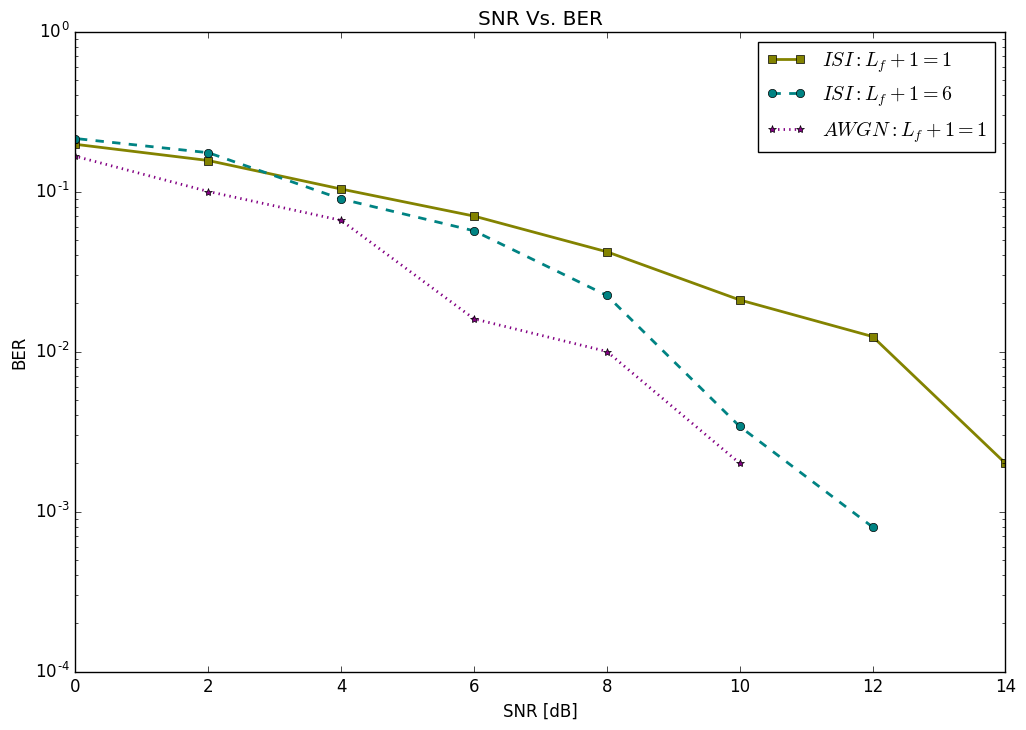
\includegraphics[scale=0.35]{img/SNR.png}
\caption{Bit-error rate VS SNR}
\label{BER}
\end{figure}


As we can see on the figure \ref{BER}, the bit-error rate is decreasing when the SNR increase(in absolute value).
Moreover, the error is much less with an equalizer length of 6 then  of 1


\subsection{What happens to the received signal constellation when you set the equalizer length to one?}

After a little bit of thinking, we can make the assumption that if we increase the length of the equalizer, the result will become better and better. In fact, we have the following theorical formula. 

\begin{equation}
\sum_{l=0}^{L_f}f[l]\hat{h}[n-l]\approx \delta [n-n_d]
\label{equ1}
\end{equation}

As we can see in the equation \ref{equ1}, we are estimating the parameter $f$, the filter which is being used to remove the interference symbol of the received signal coming from the channel canal. And if we increase the size of terms for the filter, we will have a better result. Now, we can validate that assumption thanks to the simulation. Here is the results.

%\begin{figure}[ht]
    \begin{minipage}[b]{0.48\linewidth}
        \centering 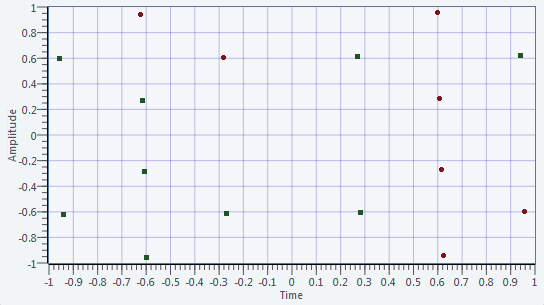
\includegraphics[scale=0.55]{img/ISI-1.png}
    \captionof{figure}{\label{fig1}Constellation for an equalizer length of 1}
    
    \end{minipage}\hfill
    \begin{minipage}[b]{0.48\linewidth}
         \centering 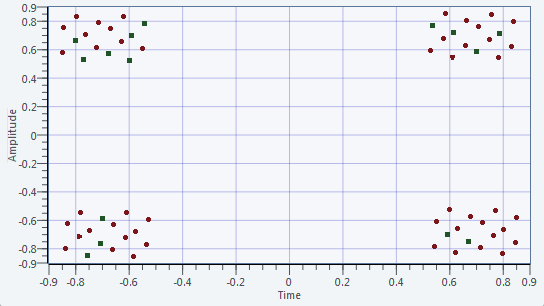
\includegraphics[scale=0.55]{img/ISI-2.png}
        \captionof{figure}{\label{fig2}Constellation for an equalizer length of 2}
    \end{minipage}
    \begin{minipage}[b]{0.48\linewidth}
        \centering 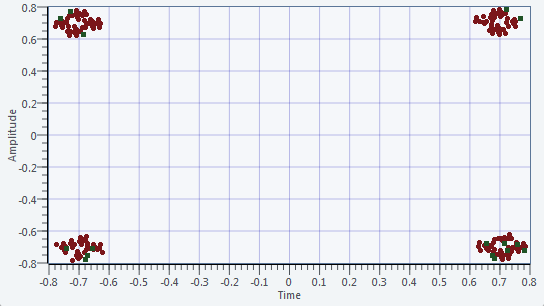
\includegraphics[scale=0.55]{img/ISI-3.png}
    \captionof{figure}{\label{fig3}Constellation for an equalizer length of 3}
    
    \end{minipage}\hfill
    \begin{minipage}[b]{0.48\linewidth}
         \centering 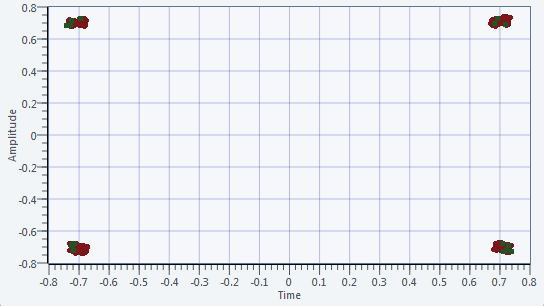
\includegraphics[scale=0.55]{img/ISI-4.png}
        \captionof{figure}{\label{fig4}Constellation for an equalizer length of 4}
    \end{minipage}
    
    \begin{minipage}[b]{0.48\linewidth}
        \centering 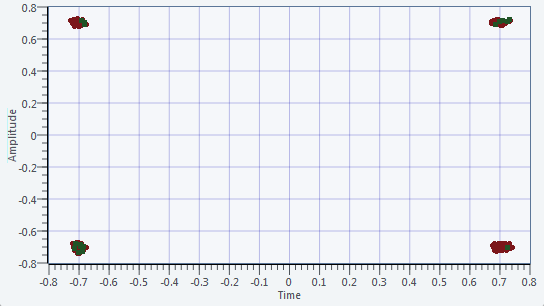
\includegraphics[scale=0.55]{img/ISI-5.png}
    \captionof{figure}{\label{fig5}Constellation for an equalizer length of 5}
    
    \end{minipage}\hfill
    \begin{minipage}[b]{0.48\linewidth}
         \centering 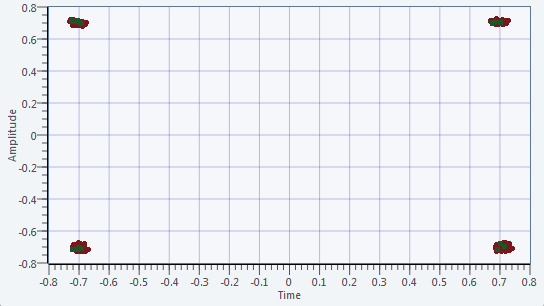
\includegraphics[scale=0.6]{img/ISI-6.png}
        \captionof{figure}{\label{fig6}Constellation for an equalizer length of 6}
    \end{minipage}
%\end{figure}

After a short observation of the figure \ref{fig1} to \ref{fig6}, we can check the assumption that has been done before is correct. 


\newpage
\section{Question for the lab}

\subsection{What is the symbol rate of your system?}

First we use the following formula

\begin{equation}
T_s=N*T_N in [Symbol/s]
\end{equation}

with N which is the oversampling factor and $T_N$, the sample rate. At the end, the symbol rate must remain constant. So, for $T_s=2M Sample/s$, and $N=20$, \textbf{$T_N=100 kSymbol/s$}

\subsection{What is the passband bandwidth of your system?}

The bandwidth is 40 MHz.

\subsection{Based on your observations, describe the impairments imparted to the received constellation}

\begin{figure}[ht!]
\centering
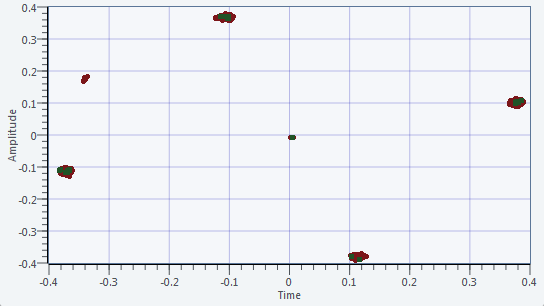
\includegraphics[scale=0.9]{img/USRP-Rotate.png}
\caption{Constellation of the received signal when the channel of the USRP is being used}
\label{usrp}
\end{figure}

On the figure \ref{usrp}, we can observe 2 things:

\begin{itemize}

\item First, the constellation has rotated. this phenoma could maybe come from a phase shift introduced in the received signal through the channel canal. We could make a link with the previous lab, which consisted of estimate the phase shift.

\item Second, the amplitude has decreased. In fact, in theory, for a QAM constellation, the magnitude is $\approx 0.7 [dB]$. On the figure \ref{usrp}, we have a magnitude of $\approx 0.4 [dB]$. We can deduce that we have an attenuation due to the canal, in other word a loss of power of the signal.

\end{itemize}

\end{document}
